\documentclass[9pt]{article}
\usepackage{fullpage}
\usepackage{amsmath}
\usepackage{amssymb}
\usepackage{graphics}
\usepackage[usenames]{color}
\usepackage{hyperref}
\usepackage{graphicx,wrapfig}
\usepackage{wallpaper}
\usepackage[inline]{enumitem}
%\usepackage{caption}

\newcommand{\addphoto}[2]{%
  \smash{%
    \makebox[0pt][l]{%
      \raisebox{#1mm}{%
        \hspace{#2mm}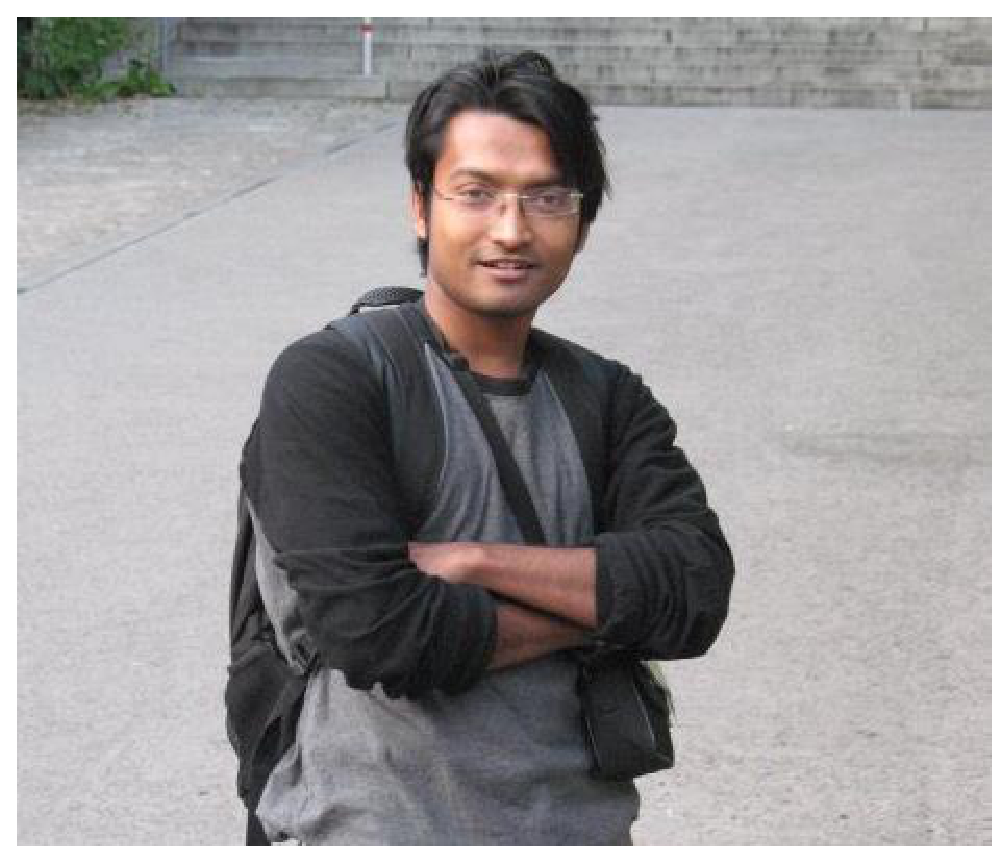
\includegraphics[scale=1]{mypic_1}%
      }%
     }%
  }%
}
\hypersetup{
    colorlinks=true,
    citecolor=blue,%
    filecolor=blue,%
    linkcolor=blue,%
    urlcolor=blue
}


\leftmargin=0.25in
\oddsidemargin=0.25in
\textwidth=6.0in
\topmargin=-0.25in
\textheight=9.25in
\newcommand{\p}{p{8cm}}

\raggedright

\pagenumbering{arabic}

\def\bull{\vrule height 0.8ex width .7ex depth -.1ex }
% DEFINITIONS FOR RESUME

\newenvironment{changemargin}[2]{%
  \begin{list}{}{%
    \setlength{\topsep}{0pt}%
    \setlength{\leftmargin}{#1}%
    \setlength{\rightmargin}{#2}%
    \setlength{\listparindent}{\parindent}%
    \setlength{\itemindent}{\parindent}%
    \setlength{\parsep}{\parskip}%
  }%
  \item[]}{\end{list}
}

\newcommand{\lineover}{
	\begin{changemargin}{-0.05in}{-0.05in}
		\vspace*{-8pt}
		\hrulefill \\
		\vspace*{-2pt}
	\end{changemargin}
}

\newcommand{\header}[1]{
	\begin{changemargin}{-0.5in}{-0.5in}
		\scshape{#1}\\
  	\lineover
	\end{changemargin}
}

\newcommand{\cmnt}[1]{}

\newcommand{\contact}[4]{
	\begin{changemargin}{-0.5in}{-0.5in}
		\begin{center}
			{\Large \scshape {#1}}\\ \smallskip
			{#2}\\ \smallskip
			{#3}\\ \smallskip
			{#4}\smallskip
		\end{center}
	\end{changemargin}
}

\newenvironment{body} {
	\vspace*{-16pt}
	\begin{changemargin}{-0.25in}{-0.5in}
  }
	{\end{changemargin}
}

\newcommand{\school}[4]{
	\textbf{#1} \hfill \emph{#2\\}
	#3\\
	#4\\
}

\makeatletter
\newcommand{\inlineitem}[1][]{%
\ifnum\enit@type=\tw@
    {\descriptionlabel{#1}}
  \hspace{\labelsep}
\else
  \ifnum\enit@type=\z@
       \refstepcounter{\@listctr}\fi
    \quad\@itemlabel\hspace{\labelsep}
\fi}
\makeatother


% END RESUME DEFINITIONS

\begin{document}

%%%%%%%%%%%%%%%%%%%%%%%%%%%%%%%%%%%%%%%%%%%%%%%%%%%%%%%%%%%%%%%%%%%%%%%%%%%%%%%%
% Name
	\begin{changemargin}{-0.5in}{-0.5in}
\begin{center}
 {\Large Swetosree Sinha} \\
 {{\texttt{Email}:\,\,\;\;\, swetosweet@gmail.com}} \\
 {{\texttt{Phone}:\;\;\,   (+1) 2179049720}} \\
\end{center}

\end{changemargin}


%%%%%%%%%%%%%%%%%%%%%%%%%%%%%%%%%%%%%%%%%%%%%%%%%%%%%%%%%%%%%%%%%%%%%%%%%%%%%%%%
% Objective
\header{Skills}
\begin{body}
	\vspace{14pt}
	\begin{itemize} \itemsep -0pt
    \item Oracle Core Database Administration (DBA)
    \item UNIX OS and system utilities
    \item Python, C Programming Language
    \item Proficient in Oracle DB management, DB Configuration, Backup/Recovery Planning, Cloning, space management and worked extensively on features like Oracle 12c \& Oracle Real Application Clusters (RAC), Recovery Manager (RMAN), Data Guard, Oracle Enterprise manager (OEM).
	  \end{itemize}

        \medskip
\end{body}


\smallskip


%%%%%%%%%%%%%%%%%%%%%%%%%%%%%%%%%%%%%%%%%%%%%%%%%%%%%%%%%%%%%%%%%%%%%%%%%%%%%%%%
% Education
\header{Career Overview}

\begin{body}
	\vspace{14pt}

	\textbf{4.10 years of industrial experience in  {\emph{\href{https://www.accenture.com/in-en/accenture-services-private-limited}{Accenture Services Pvt. Ltd.}}}} \hfill \emph{August 2012 - May 2017} \\
	\begin{itemize} \itemsep -0pt
            \item  Worked with clients \textbf{\emph{\href{http://www.libertyglobal.com}{Liberty Global}}} (Europe) \& \textbf{\emph{\href{https://www.globalpaymentsinc.com/en-us}{Global Payments Inc.}}} (USA) on diverse projects as ``Oracle Database Operation Analyst'' \& ``Unix Admin'.
            \item Proficient in creating Database through scripts, DBCA, Backup (configuration, new
script, restoration \& recover), Recovery Manager, RMAN (configuration, restore,
recover), Data Guard (configuration \& synchronization), Oracle Real Application
Clusters (RAC) activity, Oracle Enterprise Manager \& 12c activities.
            \item Proficient in Environment Build (both Unix and Windows Platform) \& System Utilities
(like debugger, profilers).
            \item Worked as part of CSR (Corporate Social Responsibility) activity.
        \end{itemize}

  \medskip
	\textbf{Bachelor of Technology in Electronics and Communication Engineering -- 85.5/100.00} \hfill \emph{August 2008 - July 2012} \\
	\textbf{\emph{\href{http://www.aecwb.edu.in/index.php/}{Asansol Engineering College}}, West Bengal, India.}\\
\end{body}

\smallskip

%%%%%%%%%%%%%%%%%%%%%%%%%%%%%%%%%%%%%%%%%%%%%%%%%%%%%%%%%%%%%%%%%%%%%%%%%%%%%%%%
%Professional Experience
\header{Professional Experience}
\begin{body}
	\vspace{14pt}
        \textbf{Role:} Database Operation Analyst \textbf{Client:} \textbf{\emph{\href{https://www.globalpaymentsinc.com/en-us}{Global Payments Inc.}}} \hfill \emph{December 2014 - May 2017}\\
	\vspace*{-4pt}
	\begin{itemize} \itemsep -0pt
          \item Monitoring different environments (Production, QA, Cert \& DEV) dashboard,
performed DB patching (PSU \& CPU - for standalone \& dataguard environment), and
bug patch, switchover activity.
          \item Using Recovery Manager (RMAN) configured backup, scripts scheduled in crontab,
restored, recovered backup \& broker setup.
          \item Performed Cloning activity (create a replication of prod environment to Test/Dev/Cert
environment).
          \item Supported migration activity of data center \& Go-Live.
          \item Deployed scripts in Linux/AIX to automate work for saving time.
          \item Worked on Oracle Enterprise Manager (monitored from here as well) \& 12C.
          \item New project “Heartland Payment” has been introduced. Taken knowledge transfer
from SME \& started working on RAC management.
	\end{itemize}

	\vspace*{-4pt}

        \textbf{Role:} SW/Application Tech Support Practitioner \textbf{Client:} \textbf{\emph{\href{http://www.libertyglobal.com}{Liberty Global}}} \hfill \emph{August 2012 - November 2014}\\
	\vspace*{-4pt}
	\begin{itemize} \itemsep -0pt
          \item Worked as part of Environment Management Team.
          \item Performed Environment build and refresh for different Releases \& Database cloning.
          \item Performing patch reviews, patch installations and patch deliveries.
          \item Providing support for releases at all stages until Go – Lives, Planning and scheduling
backup jobs using crontab.
          \item Implemented and supported oracle database and application environment
management activities.
          \item Implemented Environment build/refresh through Nolio Automation Tool.
          \item Worked on Putty \& Citrix (Remote Administration tool) using FTP, SFTP \& SCP
Protocol (For network file transfer application) for different Application Server (DEV,
MT, JIT, UAT, ORT, Prod).
	\end{itemize}

\end{body}

\smallskip

\header{Academics}
\begin{body}
\smallskip
\begin{table}[h]
\centering
\begin{tabular}{|l|l|c|c|}
\hline
\multicolumn{1}{|c|}{\textbf{University/College}} & \multicolumn{1}{c|}{\textbf{Degree}}  & \textbf{Percentage Obtained} & \textbf{Year} \\ \hline
Asansol EnginerignCollege                         & Bachelor of Technology                & 85.5\%                       & 7/2012        \\ \hline
Belrui N.G. Institution                           & West Bengal Higher SecondaryEducation & 82\%                       & 5/2008        \\ \hline
J K D U B School                                  & West Bengal Secondary Education       & 89.6\%                       & 6/2006        \\ \hline
\end{tabular}
\end{table}

\end{body}

\smallskip

\header{Achievements/Distinctions}
\begin{body}
	\vspace{14pt}
	\begin{itemize} \itemsep -0pt  % reduce space between items
            \item   Got ``Rising Star'' Award from Accenture on 2013 (September).
            \item   Got certificate from IIT Bombay for Robotics on 2010.
	\end{itemize}
\end{body}

\smallskip



\end{document}
